%%%%%%%%%%%%%%%%%%%%%%%%%%%%%%%%%%%%%%%%%
% Masters/Doctoral Thesis 
% LaTeX Template
% Version 2.4 (22/11/16)
%
% This template has been downloaded from:
% http://www.LaTeXTemplates.com
%
% Version 2.x major modifications by:
% Vel (vel@latextemplates.com)
%
% This template is based on a template by:
% Steve Gunn (http://users.ecs.soton.ac.uk/srg/softwaretools/document/templates/)
% Sunil Patel (http://www.sunilpatel.co.uk/thesis-template/)
%
% Template license:
% CC BY-NC-SA 3.0 (http://creativecommons.org/licenses/by-nc-sa/3.0/)
%
%%%%%%%%%%%%%%%%%%%%%%%%%%%%%%%%%%%%%%%%%

%----------------------------------------------------------------------------------------
%	PACKAGES AND OTHER DOCUMENT CONFIGURATIONS
%----------------------------------------------------------------------------------------

\documentclass[
11pt, % The default document font size, options: 10pt, 11pt, 12pt
%oneside, % Two side (alternating margins) for binding by default, uncomment to switch to one side
english, % ngerman for German
singlespacing, % Single line spacing, alternatives: onehalfspacing or doublespacing
%draft, % Uncomment to enable draft mode (no pictures, no links, overfull hboxes indicated)
%nolistspacing, % If the document is onehalfspacing or doublespacing, uncomment this to set spacing in lists to single
%liststotoc, % Uncomment to add the list of figures/tables/etc to the table of contents
%toctotoc, % Uncomment to add the main table of contents to the table of contents
%parskip, % Uncomment to add space between paragraphs
%nohyperref, % Uncomment to not load the hyperref package
headsepline, % Uncomment to get a line under the header
%chapterinoneline, % Uncomment to place the chapter title next to the number on one line
%consistentlayout, % Uncomment to change the layout of the declaration, abstract and acknowledgements pages to match the default layout
]{MastersDoctoralThesis} % The class file specifying the document structure

\usepackage[utf8]{inputenc} % Required for inputting international characters
\usepackage[T1]{fontenc} % Output font encoding for international characters

\usepackage{palatino} % Use the Palatino font by default

\usepackage[backend=bibtex,style=authoryear,natbib=true]{biblatex} % Use the bibtex backend with the authoryear citation style (which resembles APA)

\addbibresource{example.bib} % The filename of the bibliography

\usepackage[autostyle=true]{csquotes} % Required to generate language-dependent quotes in the bibliography

%----------------------------------------------------------------------------------------
%	MARGIN SETTINGS
%----------------------------------------------------------------------------------------

\geometry{
	paper=a4paper, % Change to letterpaper for US letter
	inner=2.5cm, % Inner margin
	outer=3.8cm, % Outer margin
	bindingoffset=.5cm, % Binding offset
	top=1.5cm, % Top margin
	bottom=1.5cm, % Bottom margin
	%showframe, % Uncomment to show how the type block is set on the page
}

%----------------------------------------------------------------------------------------
%	THESIS INFORMATION
%----------------------------------------------------------------------------------------

\thesistitle{Thesis Title} % Your thesis title, this is used in the title and abstract, print it elsewhere with \ttitle
\supervisor{} % Your supervisor's name, this is used in the title page, print it elsewhere with \supname
\examiner{} % Your examiner's name, this is not currently used anywhere in the template, print it elsewhere with \examname
\degree{Bachelor Of Science} % Your degree name, this is used in the title page and abstract, print it elsewhere with \degreename
\author{Julian Nowainski} % Your name, this is used in the title page and abstract, print it elsewhere with \authorname
\addresses{} % Your address, this is not currently used anywhere in the template, print it elsewhere with \addressname

\subject{} % Your subject area, this is not currently used anywhere in the template, print it elsewhere with \subjectname
\keywords{} % Keywords for your thesis, this is not currently used anywhere in the template, print it elsewhere with \keywordnames
\university{\href{http://www.university.com}{University of Bielefeld}} % Your university's name and URL, this is used in the title page and abstract, print it elsewhere with \univname
\department{a} % Your department's name and URL, this is used in the title page and abstract, print it elsewhere with \deptname
\group{\href{http://researchgroup.university.com}{AG NI}} % Your research group's name and URL, this is used in the title page, print it elsewhere with \groupname
\faculty{\href{http://faculty.university.com}{Faculty of Technology}} % Your faculty's name and URL, this is used in the title page and abstract, print it elsewhere with \facname

\AtBeginDocument{
\hypersetup{pdftitle=\ttitle} % Set the PDF's title to your title
\hypersetup{pdfauthor=\authorname} % Set the PDF's author to your name
\hypersetup{pdfkeywords=\keywordnames} % Set the PDF's keywords to your keywords
}

\begin{document}

\frontmatter % Use roman page numbering style (i, ii, iii, iv...) for the pre-content pages

\pagestyle{plain} % Default to the plain heading style until the thesis style is called for the body content

%----------------------------------------------------------------------------------------
%	TITLE PAGE
%----------------------------------------------------------------------------------------

\begin{titlepage}
\begin{center}

\vspace*{.06\textheight}
{\scshape\LARGE \univname\par}\vspace{1.5cm} % University name
\textsc{\Large Bachelor Thesis}\\[0.5cm] % Thesis type

\HRule \\[0.4cm] % Horizontal line
{\huge \bfseries \ttitle\par}\vspace{0.4cm} % Thesis title
\HRule \\[1.5cm] % Horizontal line
 
\begin{minipage}[t]{0.4\textwidth}
\begin{flushleft} \large
\emph{Author:}\\
\href{http://www.johnsmith.com}{\authorname} % Author name - remove the \href bracket to remove the link
\end{flushleft}
\end{minipage}
\begin{minipage}[t]{0.4\textwidth}
\begin{flushright} \large
\emph{Supervisor:} \\
\href{http://www.jamessmith.com}{\supname} % Supervisor name - remove the \href bracket to remove the link  
\end{flushright}
\end{minipage}\\[3cm]
 
\vfill

\large \textit{A thesis submitted in fulfillment of the requirements\\ for the degree of \degreename}\\[0.3cm] % University requirement text
\textit{in the}\\[0.4cm]
\groupname\\\deptname\\[2cm] % Research group name and department name
 
\vfill

{\large \today}\\[4cm] % Date
%\includegraphics{Logo} % University/department logo - uncomment to place it
 
\vfill
\end{center}
\end{titlepage}

%----------------------------------------------------------------------------------------
%	DECLARATION PAGE
%----------------------------------------------------------------------------------------

\begin{declaration}
\addchaptertocentry{\authorshipname} % Add the declaration to the table of contents
\noindent I, \authorname, declare that this thesis titled, \enquote{\ttitle} and the work presented in it are my own. I confirm that:

\begin{itemize} 
\item This work was done wholly or mainly while in candidature for a research degree at this University.
\item Where any part of this thesis has previously been submitted for a degree or any other qualification at this University or any other institution, this has been clearly stated.
\item Where I have consulted the published work of others, this is always clearly attributed.
\item Where I have quoted from the work of others, the source is always given. With the exception of such quotations, this thesis is entirely my own work.
\item I have acknowledged all main sources of help.
\item Where the thesis is based on work done by myself jointly with others, I have made clear exactly what was done by others and what I have contributed myself.\\
\end{itemize}
 
\noindent Signed:\\
\rule[0.5em]{25em}{0.5pt} % This prints a line for the signature
 
\noindent Date:\\
\rule[0.5em]{25em}{0.5pt} % This prints a line to write the date
\end{declaration}

\cleardoublepage

%----------------------------------------------------------------------------------------
%	QUOTATION PAGE
%----------------------------------------------------------------------------------------


%----------------------------------------------------------------------------------------
%	ABSTRACT PAGE
%----------------------------------------------------------------------------------------

\begin{abstract}
\addchaptertocentry{\abstractname} % Add the abstract to the table of contents
The Thesis Abstract is written here (and usually kept to just this page). The page is kept centered vertically so can expand into the blank space above the title too\ldots
\end{abstract}

%----------------------------------------------------------------------------------------
%	ACKNOWLEDGEMENTS
%----------------------------------------------------------------------------------------

%----------------------------------------------------------------------------------------
%	LIST OF CONTENTS/FIGURES/TABLES PAGES
%----------------------------------------------------------------------------------------

\tableofcontents % Prints the main table of contents

%\listoffigures % Prints the list of figures

%\listoftables % Prints the list of tables

%----------------------------------------------------------------------------------------
%	ABBREVIATIONS
%----------------------------------------------------------------------------------------



%----------------------------------------------------------------------------------------
%	PHYSICAL CONSTANTS/OTHER DEFINITIONS
%----------------------------------------------------------------------------------------



%----------------------------------------------------------------------------------------
%	SYMBOLS
%----------------------------------------------------------------------------------------



%----------------------------------------------------------------------------------------
%	DEDICATION
%----------------------------------------------------------------------------------------


%----------------------------------------------------------------------------------------
%	THESIS CONTENT - CHAPTERS
%----------------------------------------------------------------------------------------

\mainmatter % Begin numeric (1,2,3...) page numbering

\pagestyle{thesis} % Return the page headers back to the "thesis" style

% Include the chapters of the thesis as separate files from the Chapters folder
% Uncomment the lines as you write the chapters

% Chapter 1

\chapter{Introduction} % Main chapter title

\label{Introduction} % For referencing the chapter elsewhere, use \ref{Chapter1} 

%----------------------------------------------------------------------------------------

% Define some commands to keep the formatting separated from the content 
\newcommand{\keyword}[1]{\textbf{#1}}
\newcommand{\tabhead}[1]{\textbf{#1}}
\newcommand{\code}[1]{\texttt{#1}}
\newcommand{\file}[1]{\texttt{\bfseries#1}}
\newcommand{\option}[1]{\texttt{\itshape#1}}

%----------------------------------------------------------------------------------------
\section{Motivation}
Humans are very skilled when it comes to the task of exploring objects based merely on the haptic feedback they get from touching them. In a setting with multiple objects, a desired object can be found quite fast among the others. Searching for some objects like keys in a bag, or a phone on a nightstand in the dark are some examples of a three-dimensional haptic search task. In such tasks, one searches for a desired object, called the target, amongst other objects that are not of interest called distractors. Often, it is a specific feature of an object that makes it stand out among others. These features can be, for an instance, material properties, size, weight or shape \cite{HapticShape}. This is called the pop-out effect where the target feature is then said to be salient with respect to the distractor properties. \\
This phenomenon has not only been aspect of research in the haptic domain, but rather had its beginning in the vision. An example was to find a red dot among green ones, which could be done effortlessly without the need for a throughout search. However, finding a line with a specific rotation in an image with multiple lines of various rotations takes some effort \cite{treisman_gormican_1988}. Furthermore Ledermann and Klatsky found in 1987 \cite{EPs}, that each search strategy consists of a set of patterns of explorations that are called exploratory procedures (EPs). This means that the efficiency of a haptic search is not only based on the salient target feature, but also on the search strategy that is used. This shows the complexity of haptic search tasks and makes it even more interesting that humans can do this with high accuracy and seemingly little effort.  \\
A lot of research was done to investigate human behavior in such tasks, but to this day it was merely investigated what the approaches are to implement such behavior in technical systems such as robots. This work wants to consider two questions with the data recorded in a haptic search experiment with a multimodal glove worn by participants: Is it possible to inspect these pop-out effects based on tactile data and pose-information as well as the question of the applicability of these data in machine learning tasks. 

\section{Goals} \label{Goals}
A first goal of this work was to provide a setting where haptic search tasks could be performed by participants and be recorded with suitable hardware. In section \ref{Haptic Search Experiment} the haptic search experiment will be proposed and discussed starting by the experimental setup, the execution, hardware and the overall setting.\\
After having recorded the data a second goal was aimed at generating a data set that was suitable for supervised learning tasks. These included postprocessing the raw data and generating labels for the individual trials. Section \ref{Data} describes the efforts that were made to reach this goal.\\
The last goal was to use the information collected with the data to perform machine learning tasks to investigate the differences between target- and distractor objects and measure the performance of the developed models. Section \ref{Evaluation} will describe the different experiments and models that were used to address the question for applicability of recorded data from haptic search experiments performed by humans.  

% Chapter 2

\chapter{Haptic Search Experiment} % Main chapter title

\label{Haptic Search Experiment} % For referencing the chapter elsewhere, use \ref{Haptic Search Experiment} 

%----------------------------------------------------------------------------------------
%In diesem Kapitel wird der Versuch, die benutzte Hardware , %und das komplette Setting von der Aufnahme beschrieben

%----------------------------------------------------------------------------------------
\section{Haptic Search Experiment}
\subsection{Experimental Setup}
The Modular Haptic Stimuli Board (MHSB) makes up the core part of the experiment. It is a setting with two wooden frames that hold stimuli objects. These objects are 3 x 3 cm big wooden blocks, which have a primitive three-dimensional shape on top of it or are just plane. The whole set consists of 360 blocks with 55 different shapes.\\
The first wooden frame can fit 25 objects and is used for learning a target object whereas the second frame has a capacity of 100 objects and is used for searching target objects. The stimuli are statically installed in the frames and not manipulable to allow a focus on just the search task itself (see Figure \ref{MHSBBOARDS}).\\
\\
For this experiment, a subset of stimuli was chosen, consisting of 5 different shapes and plane ones (see Figure \ref{Stimuli}). The target consists of one object and is placed central in the small frame with the rest of the space consisting of plane stimuli. The big frame contains the rest of this subset, where each shape exist 4 to 5 times, including the target. The objects were distributed mostly equally and kept the same rotation throughout the experiment. Only the distribution and the target were changed with each trial.\\

\begin{figure}[H]
	\centering
	\begin{minipage}{0.49\textwidth}
		\centering
		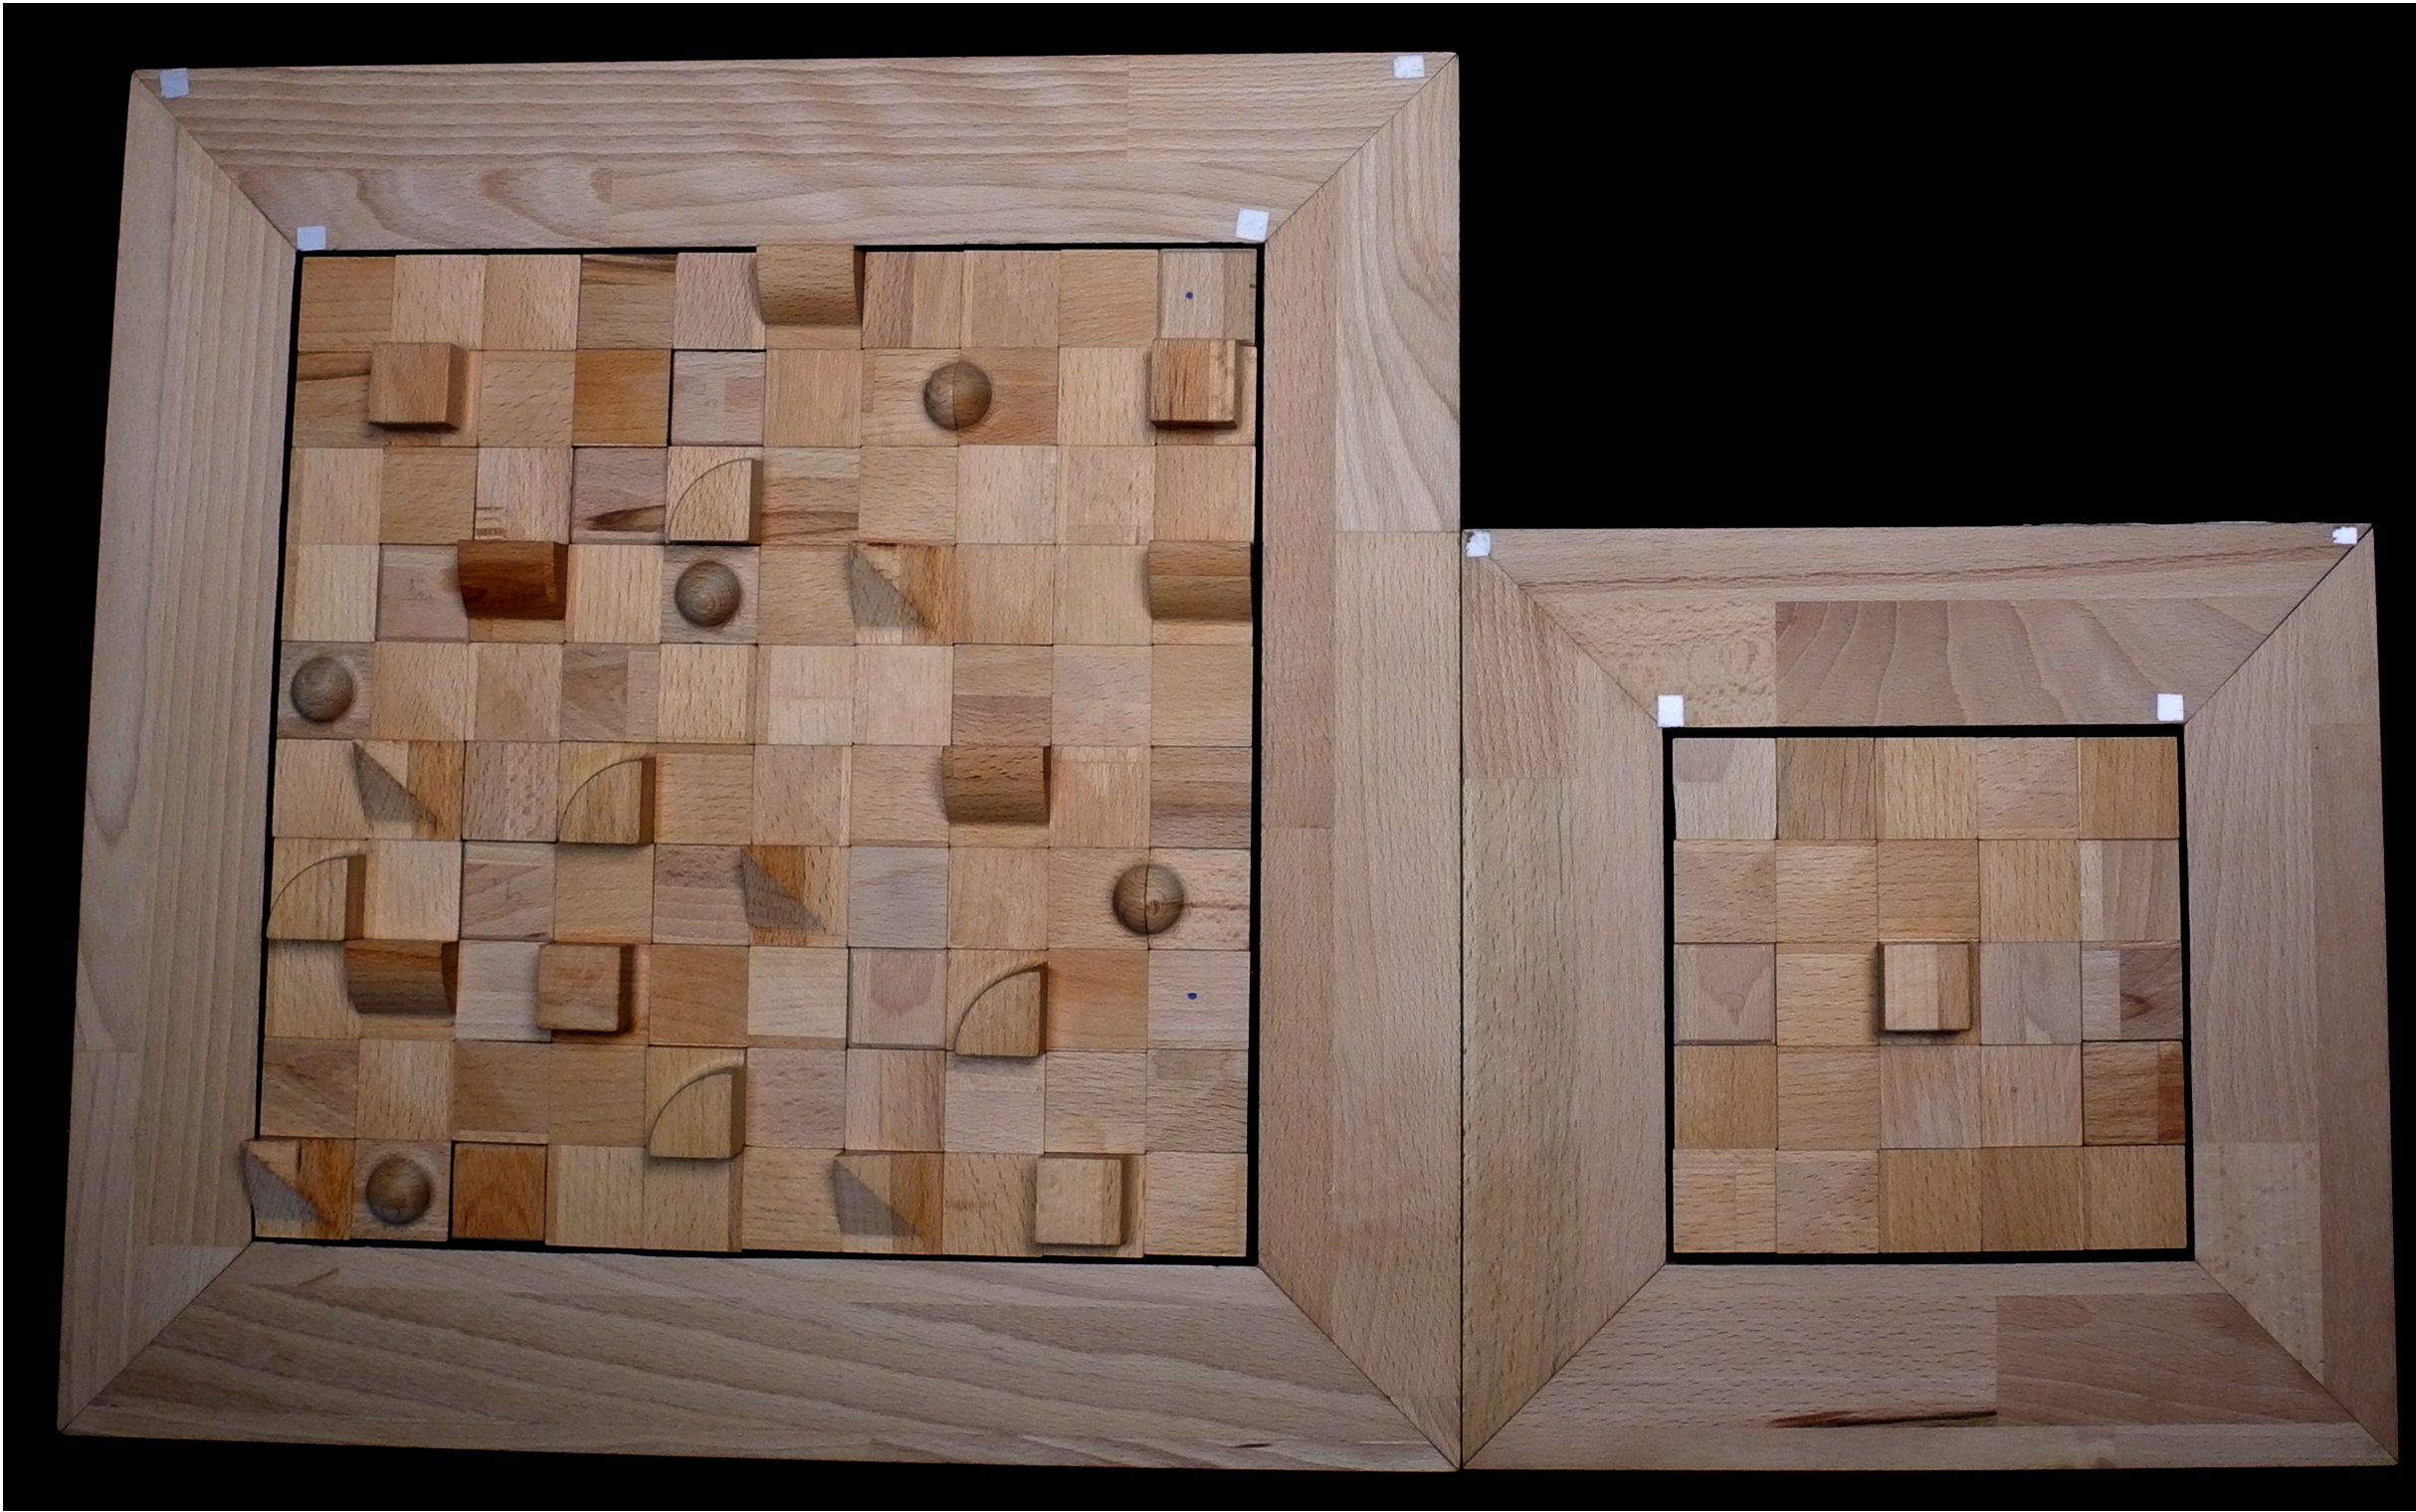
\includegraphics[width=\textwidth]{MHSB}
		\caption{MHSB: on the right side for learning, on the left for search task}
		\label{MHSBBOARDS}
	\end{minipage}
	\begin{minipage}{0.49\textwidth}
		\centering
		\includegraphics[width=0.83\textwidth]{Stimuli}
		\caption{Stimuli objects from left: Wave, Sphere, Quarter, Box, Pyramid}
		\label{Stimuli}
	\end{minipage}
\end{figure}


\subsection{Execution}  
For this experiment, 7 participants were invited and asked to solve a haptic search task while being blindfolded. The participants were 23 to 28 years old and included both genders. All participants were right-handed and have never seen the stimuli objects, so that during the task they never knew how the set of objects looked like and their perception was purely based on the haptic features.\\
Each participant performed on maximal 5 trials, where after each trial, the target was exchanged and the distribution of the stimuli on the big frame was changed. Before the beginning, there were 2 rehearsals to accustom the subjects to the setting. No participant had the same target twice or more and the task was done with just the right hand, while wearing a glove to record relevant data (See \ref{Hardware}).\\
\\
For the procedure, each participant was given a description of the task (See Appendix \ref{AppendixA}). The task consisted of two parts. \\
The first task was to explore the target object on the small frame and remembering it just by its haptic features. When collected enough information about the target stimulus, the subject should proceed to the big frame and search for the learned target. The only goal in this part was to remember the approximate position of the target and not saying that it was found or pointing at it, so the recorded data would not contain pauses or pointing postures.\\
It was not necessary to find every target shape in the big frame, just as many as one could. The time was limited to 30 seconds to guarantee that the focus lies only on the salient features. An acoustic signal by the examiner determined the start- and endpoint of the experiment.\\
The second part of the experiment was to figure out if the subjects found the target object between the non-target objects, called distractors, and how well they could remember the approximate position on the frame. Again an acoustic signal determined start and end of the trial. For the second part, the subjects had just 10 seconds left to find the targets and point on them. The short period of time was set to prevent the subjects from exploring too much of the frame and focusing only on the smallest set of haptic features that were sufficient enough to differentiate between target and distractor.\\

%----------------------------------------------------------------------------------------
\section{Hardware} \label{Hardware}
In this section the used hardware will be described as well as the overall setting that was used to record the data for the experiment.\\
There will be first a brief description of the glove that was used to capture tactile relevant and hand posture data followed by a description of the Vicon system to capture position data in a three-dimensional environment. At the end the implementation of the hardware into the experimental setting is explained.

\subsection{Glove}
A detailed explanation of the underlying technical properties and its implementation into the glove can be found in the work of Bianchi et. al. \cite{Glove}.\\
\\
To record data for this experiment, a device was needed that would be able to capture the most relevant patterns underlying a haptic search task. These so called exploratory features (EPs) describe the behavior of the hand during the exploration \cite{EPs}. Furthermore a device for recording the tactile properties was needed.\\
The multi-modal sensing glove combines both of these features. On the bottom side of the glove 64 tactile cells are mounted, covering hand palm and fingers. These fabric-based sensors record local pressures with a frequency of 150 Hz. The top side consists of 18 bending sensors, used to capture the joint angles representing the hand pose with a frequency of 50 Hz.
 
\subsection{Vicon}
For capturing the position of the hand and the MHSB, the Vicon system was used \cite{Vicon}. It records motion data with a frequency of 200 Hz, using retroreflective markers that are tracked by infrared cameras.\\
Also included is a Basler camera, generating a top-down view for the experiment.

\subsection{Setting}
To record motion data from the subjects hand, 17 reflective markers has been placed on an extra glove that the participant wears atop of the multi-modal one. The markers were placed in a position as shown in Figure \ref{Glove_markers} to guarantee a good reconstruction of the finger and hand movements.\\
The most time-consuming part was to find a setting of the Vicon cameras that would capture the reflective markers continuously, making sure to minimize the occurrence of gaps. The result is shown in Figure \ref{Setting} There were 14 Vicon cameras placed in a semicircle around the MHSB. The Basler camera was placed directly above the frames. As an addition, there were 2 cameras placed on the left and right side to record also the side-view of the experiment.\\
The glove was connected via USB and serial-port to a nearby computer. A second computer controlled the Vicon system. To simultanetly start the recording, a synchronising tool called MSS was used (See \ref{recording}).

\begin{figure}[H]
	\centering
	\begin{minipage}{0.49\textwidth}
		\centering
		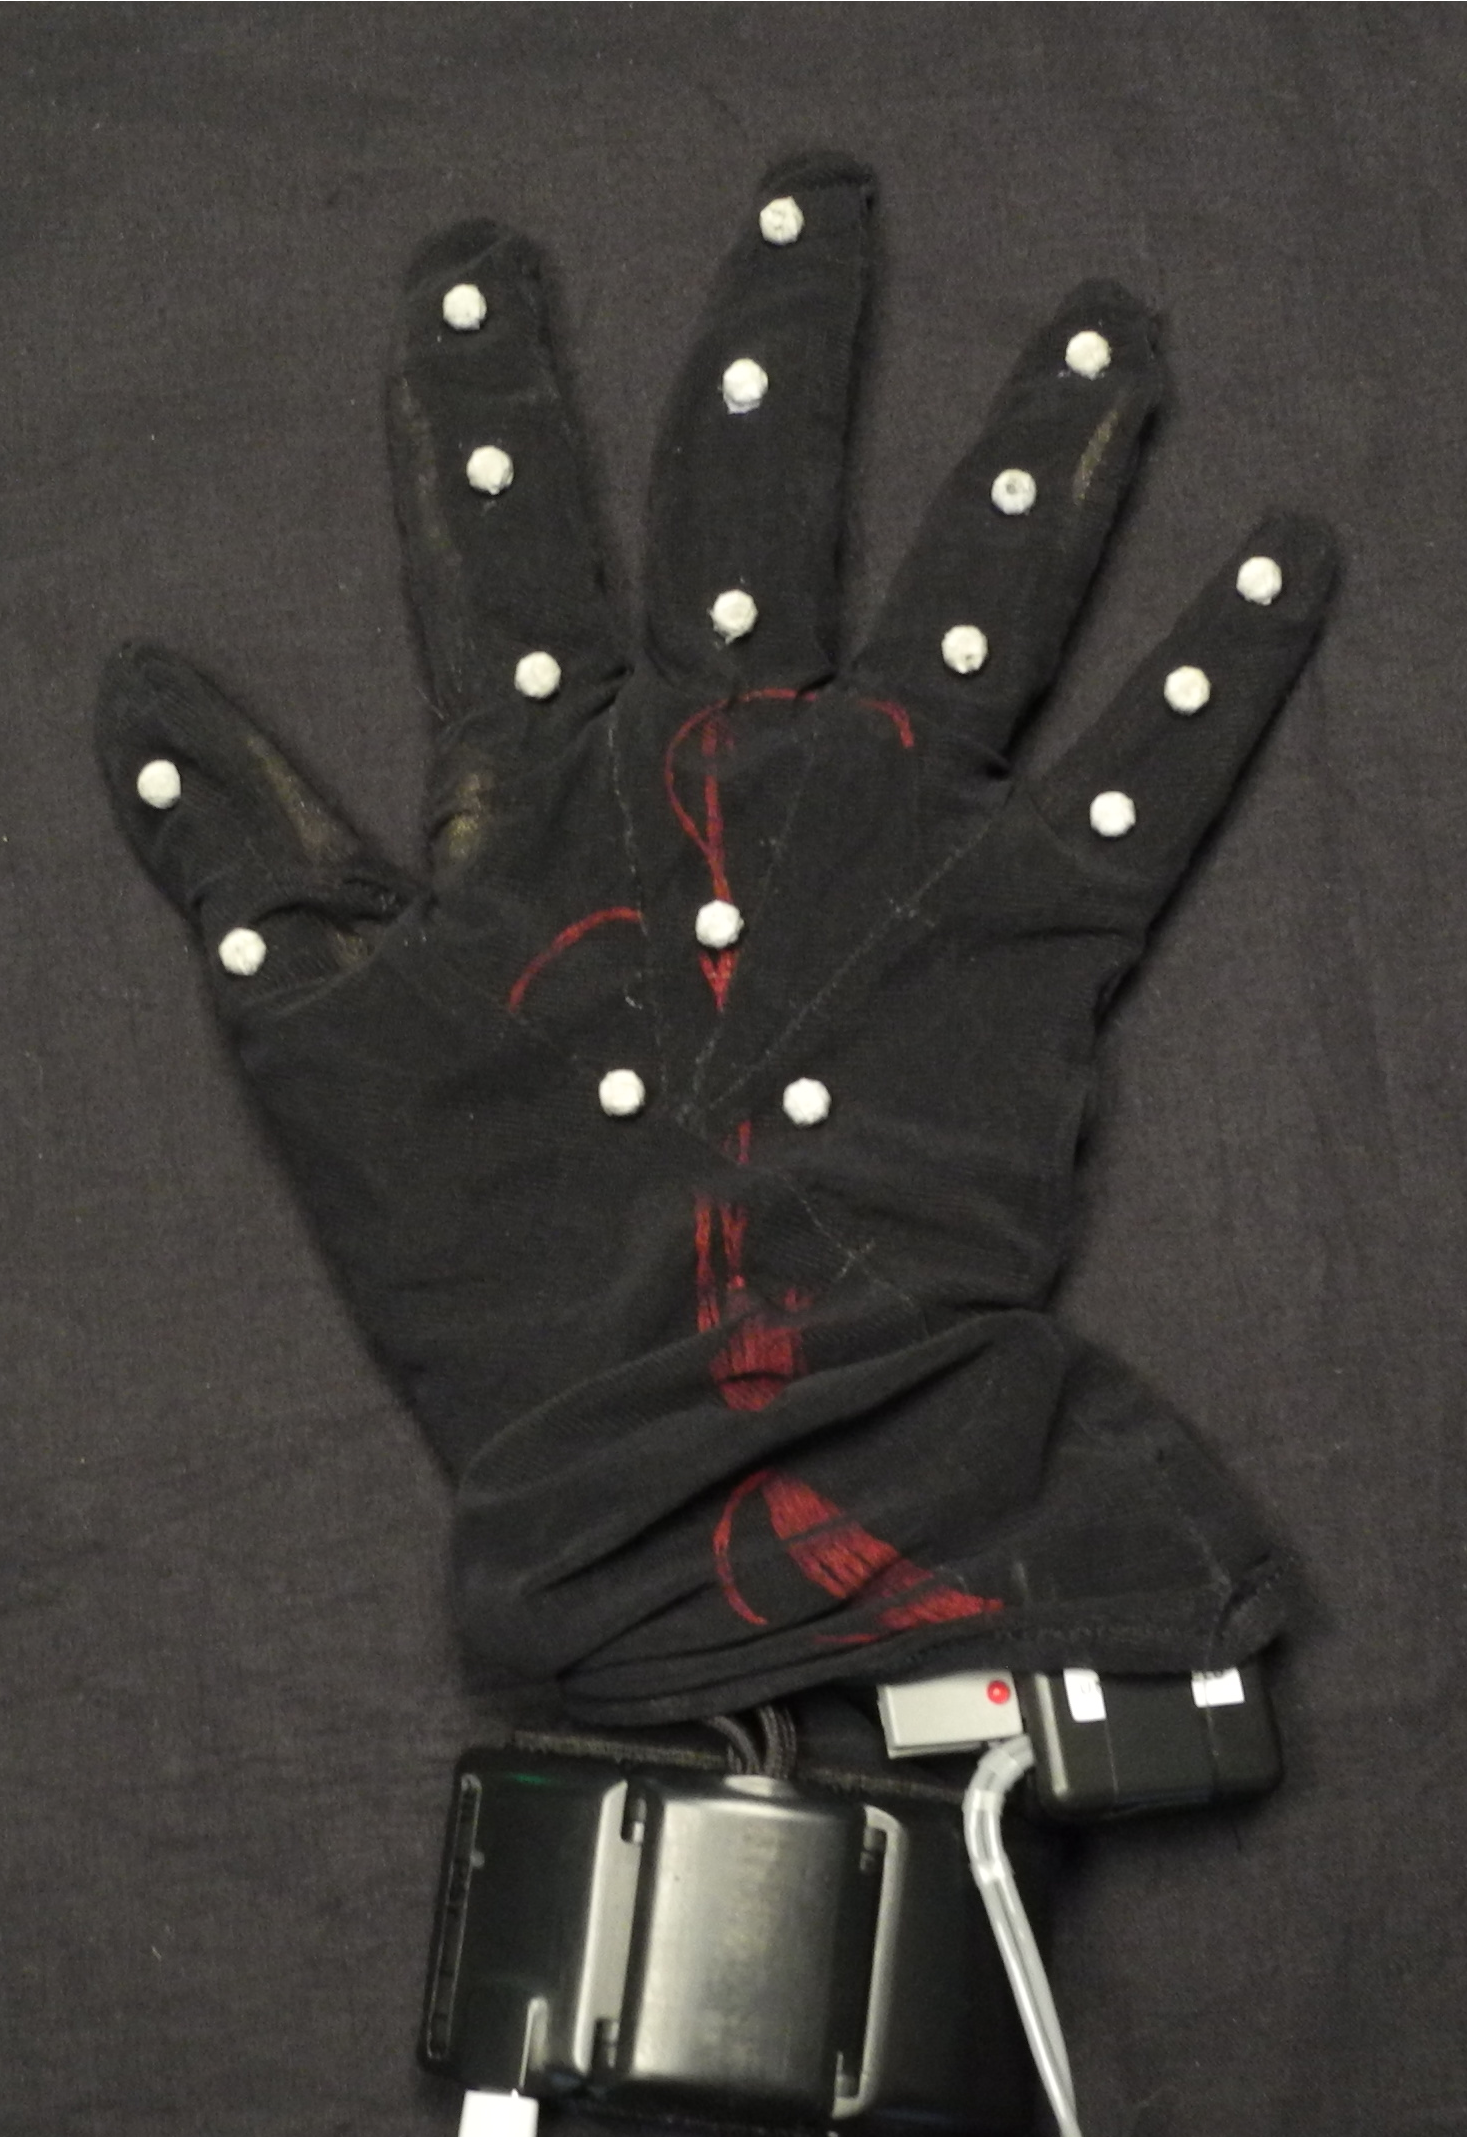
\includegraphics[width=0.55\textwidth]{glove_markers}
		\caption{Glove with 17 retroreflective markers for tracking the hand movement with Vicon}
		\label{Glove_markers}
	\end{minipage}
	\begin{minipage}{0.49\textwidth}
		\centering
		\includegraphics[width=\textwidth]{Setting}
		\caption{Experimental setting with MHSB, glove and Vicon cameras}
		\label{Setting}
	\end{minipage}
\end{figure}
  
%\include{Chapters/Chapter3}
%\include{Chapters/Chapter4} 
%\include{Chapters/Chapter5} 

%----------------------------------------------------------------------------------------
%	THESIS CONTENT - APPENDICES
%----------------------------------------------------------------------------------------

\appendix % Cue to tell LaTeX that the following "chapters" are Appendices

% Include the appendices of the thesis as separate files from the Appendices folder
% Uncomment the lines as you write the Appendices

%\chapter{Experimental Instructions} \label{AppendixA}

\begin{figure}[H]
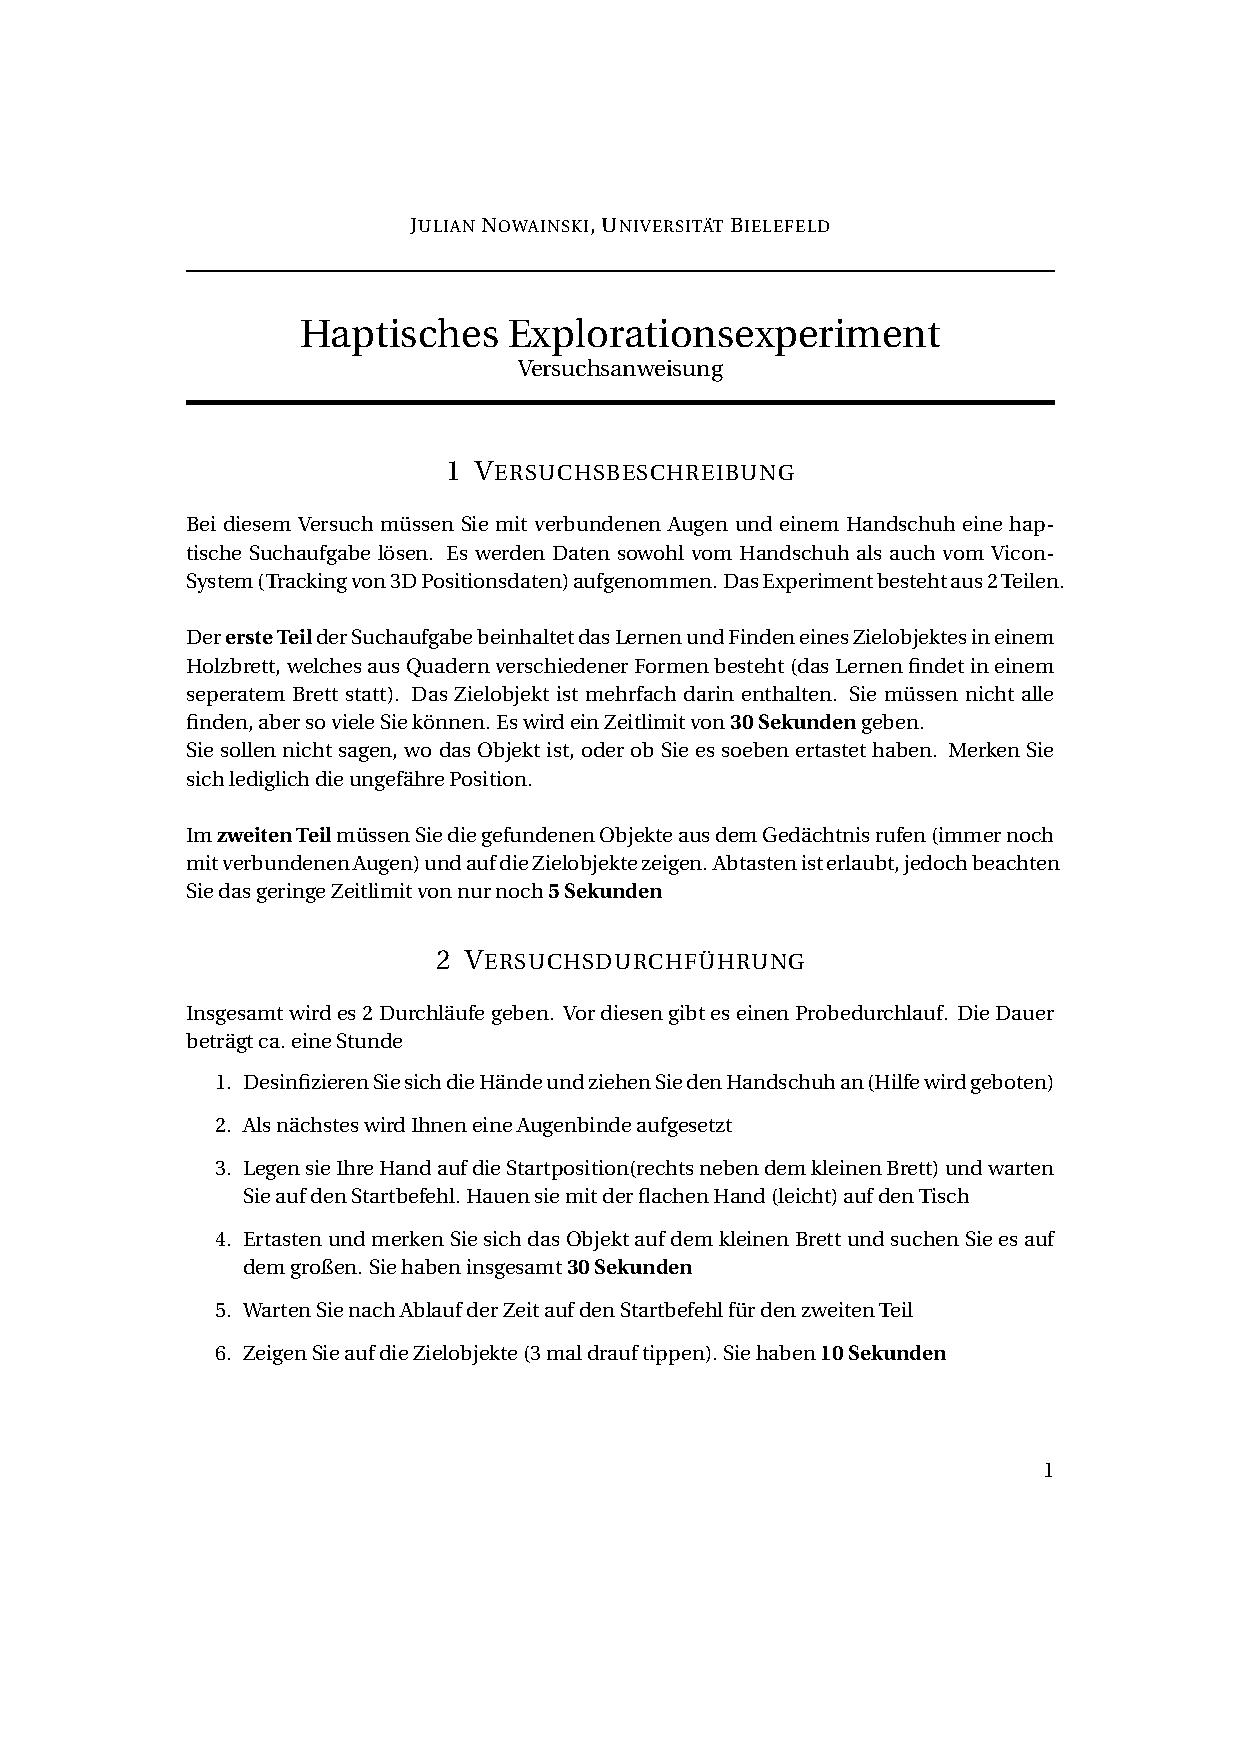
\includepdf[scale=0.9,offset=0 -80]{Appendices/instructions_ger.pdf}
\end{figure}





%\include{Appendices/AppendixB}
%\include{Appendices/AppendixC}

%----------------------------------------------------------------------------------------
%	BIBLIOGRAPHY
%----------------------------------------------------------------------------------------

\printbibliography[heading=bibintoc]

%----------------------------------------------------------------------------------------

\end{document}  
